\subsection{Quality Accessment}
In this part, all the 3D resources' quality are compared from different perspectives.
\subsubsection{Quantitative indicators}
\begin{table}[H]
	\centering
	\caption{Quantitative Evaluation of Reconstructed Objects and Background}
	\begin{tabular}{c|c|c|c|c}
		\hline
		\textbf{Object} & \textbf{PSNR $\uparrow$} & \textbf{SSIM $\uparrow$} & \textbf{LPIPS $\downarrow$} & \textbf{Training Time(min)} \\
		\hline
		A-Kobe   & 30.94 & 0.9569 & 0.2245 & 55 \\
		\hline
		B-Astronaut & - & - & - & 20 \\
		B-Bunny  & - & - & - &  20\\
		\hline
		C-Firekeeper & 11.669 & 0.1588 & 0.5905 &  60\\
		C-Robot & 8.5543 & 0.5913 & 0.4767 &  60\\
		\hline
		BG-Garden & 30.31 & 0.9080 & 0.1242 & 92 \\
		\hline
	\end{tabular}
	\label{tab:quantitative_results}
\end{table}

In this section, PSNR(Peak Signal-to-Noise Ratio),SSIM(Structural Similarity Inde),LPIPS(Learned Perceptual Ima`ge Patch Similarity) are introduced to access the quality of models. Specifically, Object Bs have no ground truth picture, so we didn't access them this way. \textbf{Also, Object Cs have only 1 picture and the rendering image is manually generated by us, so the accessment is not accurate and can only be taken for reference.}

We can see that Object A and Background Garden have obsessive advantages over Object Cs in geometry accuracy and  mesh details.


For the training time, Object B is the fastest, Object Cs all takes about an hour.
Specifically, Object A(COLMAP+2DGS) is variable.


Considering the training dynamic of Figure~\ref{figure:Feature Points}. We can see that the Garden has 128395 points compared with 5829 points of Kobe at the beginning of the training. This is because of the huge and high resolution dataset of Garden,which helps capture massive amounts of points during the COLMAP part. This takes time(1:12:42hour), but allows faster 2DGS(19:30min). 
\begin{figure}[h]
	\centering
	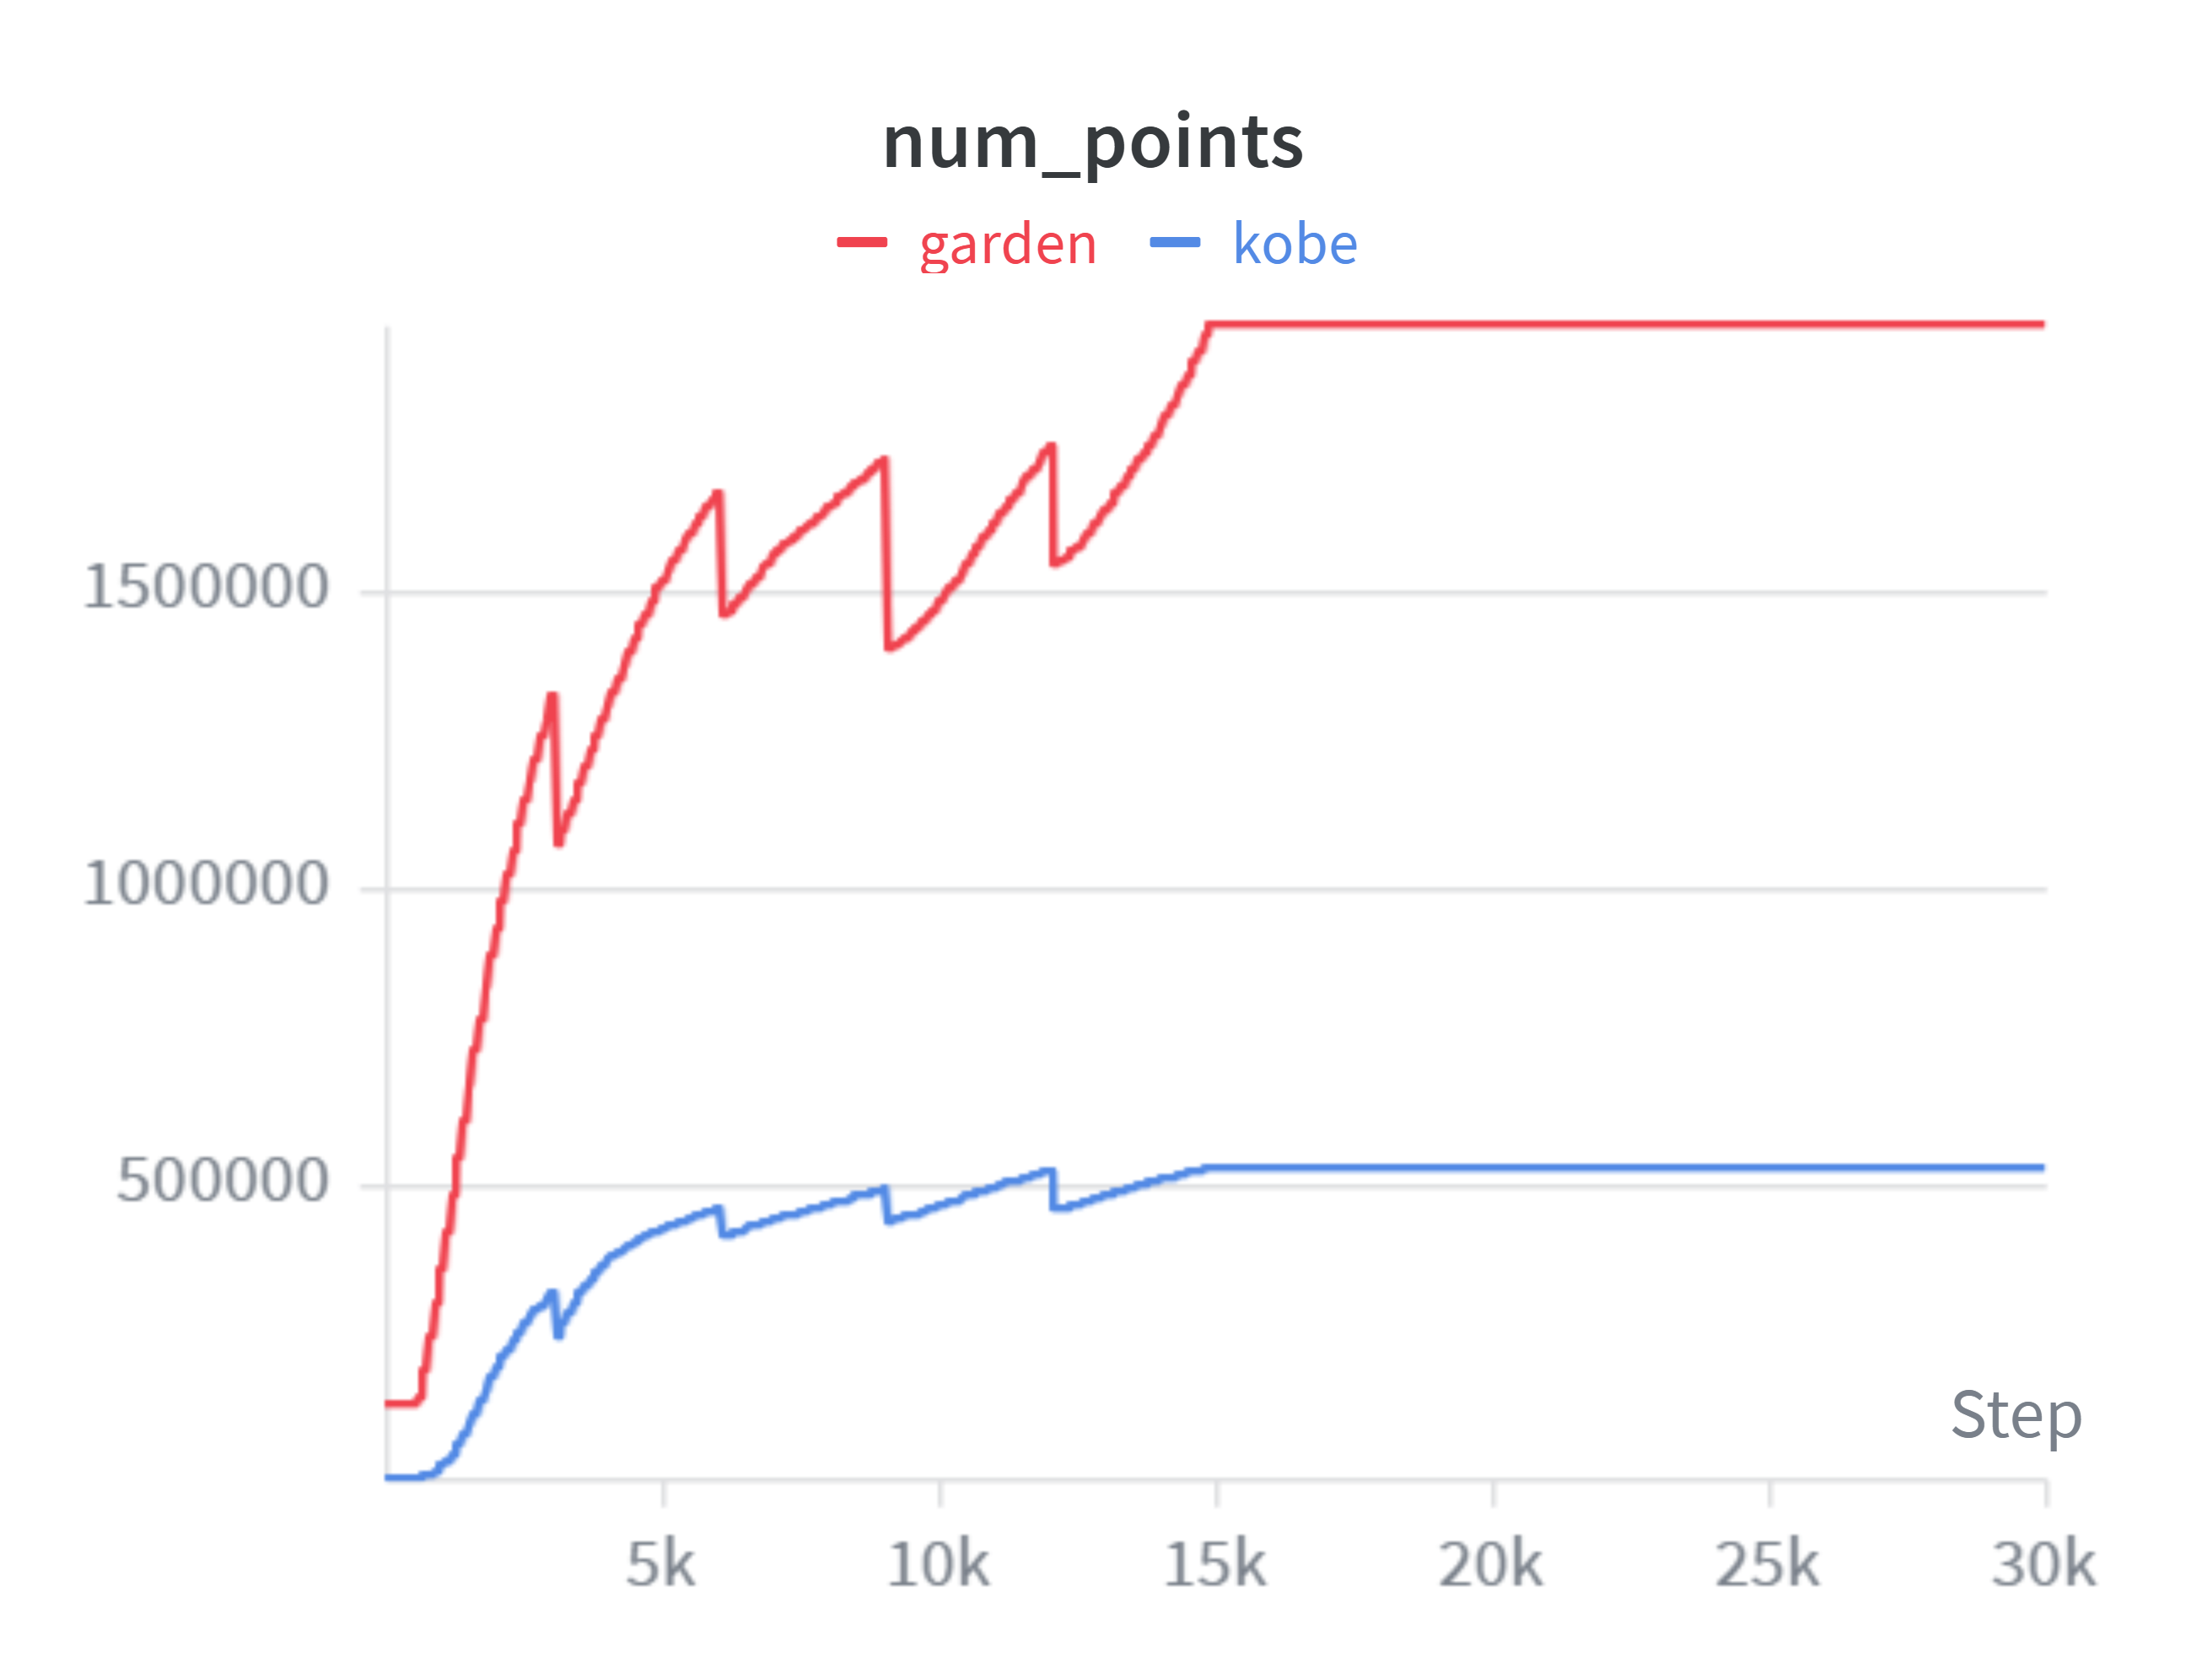
\includegraphics[width=0.4\linewidth]{figures/task1/background/num_points.png}
	\caption{Feature Points}
	\label{figure:Feature Points}
\end{figure}	


\subsubsection{Visual Evaluation}
Considering the different dataset(prompt) of different object, we also try to access the results directly through human eye,which contains some irregular meshes.This can be seen in the videos we offered in the appendix.

For Object A and Background Garden, the visualization looks good and the overall details fit very well except for the places where the pictures don't cover(outside the scene/sky/under the table).

For Object Bs, it's easy to see that the color distribution is not that appropriate as they're in the real world as Figure~\ref{Astronaut Color} Also the details are rough and unsmooth when taking a close look.

For Object Cs, the color distributions are better than Object Bs. The modeling of the front and back are relatively good. However, the side view is worse than the real view, often appearing thinner. This is because the model only receives a frontal photo of the object, making it difficult to accurately judge the thickness:Figure~\ref{fig:firekeeper_vertical} and Figure~\ref{fig:Robot_vertical}. Figure~\ref{fig:objectC_failures} show some of their flaws:
\begin{figure}[h]
	\centering
	
	% 第一组：Firekeeper
	\begin{minipage}{0.45\textwidth}
		\centering
		\textbf{Firekeeper} \\[1ex]
		\begin{subfigure}{0.45\textwidth}
			\centering
			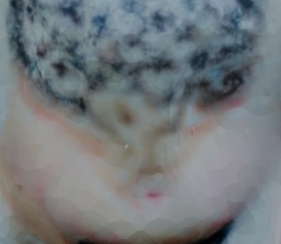
\includegraphics[width=\linewidth]{figures/task1/objectC/firekeeper_wrong_1.png}
			\caption{Mask lacks detail}
		\end{subfigure}
		\hfill
		\begin{subfigure}{0.45\textwidth}
			\centering
			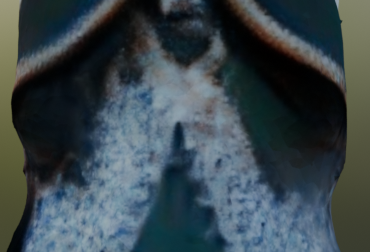
\includegraphics[width=\linewidth]{figures/task1/objectC/firekeeper_wrong_2.png}
			\caption{Hands mistaken as pattern of clothes}
		\end{subfigure}
	\end{minipage}
	\hfill
	% 第二组：Robot
	\begin{minipage}{0.45\textwidth}
		\centering
		\textbf{Robot} \\[1ex]
		\begin{subfigure}{0.45\textwidth}
			\centering
			
\includegraphics[width=\linewidth]{figures/task1/objectC/robot_wrong_1.png}
			\caption{Poor depth handling}
		\end{subfigure}
		\hfill
		\begin{subfigure}{0.45\textwidth}
			\centering
			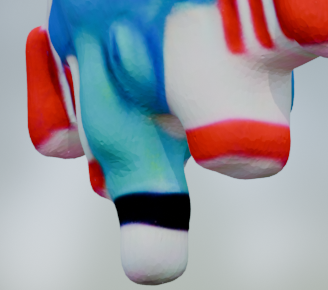
\includegraphics[width=\linewidth]{figures/task1/objectC/robot_wrong_2.png}
			\caption{Joints erased}
		\end{subfigure}
	\end{minipage}
	
	\caption{Failure cases of Object C grouped by subject.}
	\label{fig:objectC_failures}
\end{figure}

